%% This is an example first chapter.  You should put chapter/appendix that you
%% write into a separate file, and add a line \include{yourfilename} to
%% main.tex, where `yourfilename.tex' is the name of the chapter/appendix file.
%% You can process specific files by typing their names in at the 
%% \files=
%% prompt when you run the file main.tex through LaTeX.
\chapter{Docker Fundamentals}

Docker is a relatively new open-source framework that serves as a lightweight alternative to virtual machines. It provides users with the ability to create isolated, high-performing containers that can be seamlessly deployed to other hosts that are also running the Docker Engine. Unlike virtual machines, containers share the kernel with the host and therefore rely on specific features in the kernel to provide a comparable level of isolation. For now, these containers are restricted to Linux; however, Microsoft has recently made a commitment to bring container technology based on Docker to the Windows platform \cite{windows-docker}.

For the past few years, Docker has been under active heavy development and in recent months is gaining popularity across the industry. An extraordinary number of new projects and platforms are being built on top of Docker, resulting in a rich and lively ecosystem. 


In section~\ref{ch2:system}, we outline the technical details of Docker; in section~\ref{ch2:lingo}, we describe fundamental terms that will be essential to the understanding of VM2Docker; in section~\ref{ch2:usecase} we dive into the wide variety of use cases Docker containers can have; in section~\ref{ch2:industry} we discuss the industry's response to Docker; and finally in section~\ref{ch2:patterns} we discuss defacto Docker design patterns that have become popular.

\section{System Details}\label{ch2:system}
The Docker platform is divided into the Docker Engine, which supports the runtime and execution of containers, and the Docker Registry, which provides the hosting and delivery of a repository of Docker images. Each container provides a namespaced, isolated environment for execution. Docker exploits filesystem layering, as well as specific features of the Linux kernel to make all of these possible.

\begin{figure}[h]
\centering
    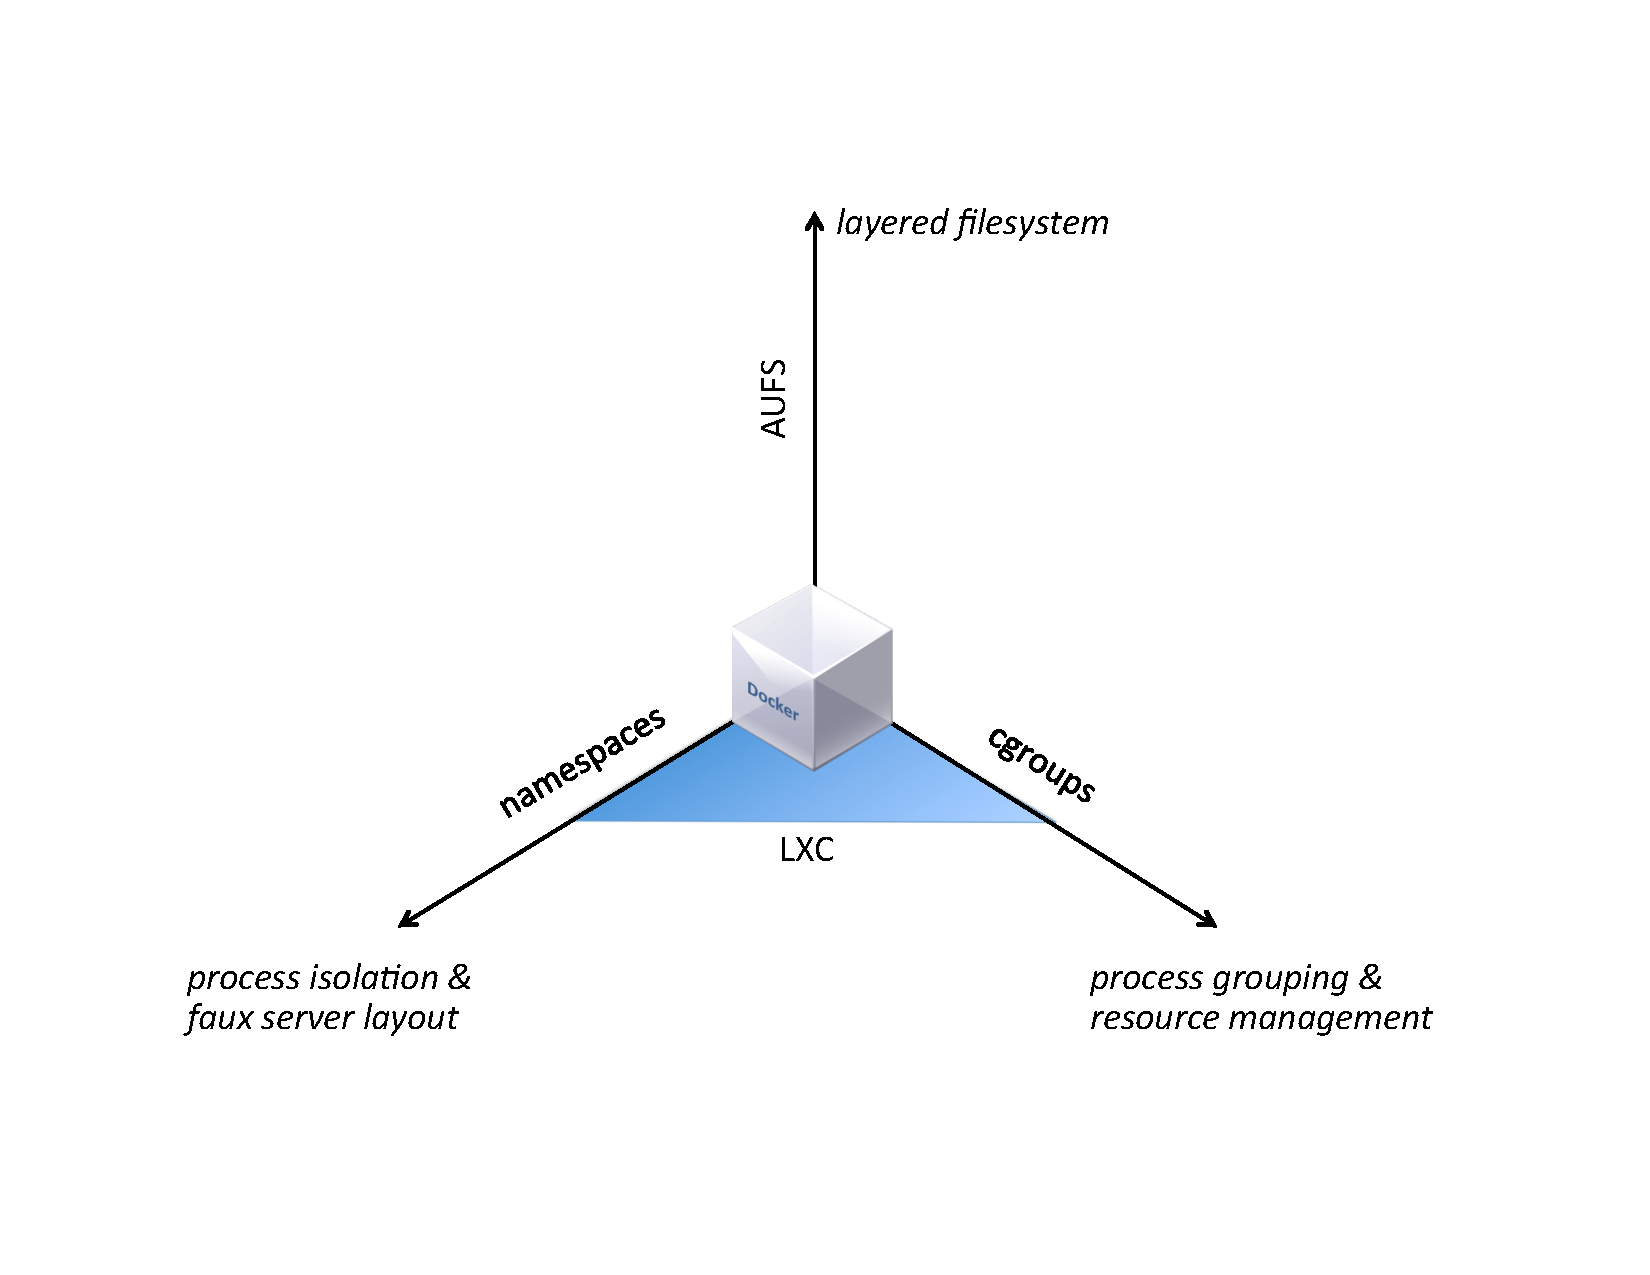
\includegraphics[width=1.0\textwidth]{docker.pdf}
    \caption{A graphic outlining the three fundamental components that make up the Docker framework. Namespace and cgroup support are provided by the LXC (LinuX Container) kernel extensions, and filesystem layering is provided by AUFS.}
\end{figure}

\subsection{cgroups}
Cgroups, or control groups, are a feature on the Linux kernel that provides resource limiting, in the form of memory or disk limits, as well as prioritization of CPU and disk throughput. These features are comparable to those offered by a virtual machine hypervisor to allocate a given amount of memory and CPU, network, and disk priority to a virtual machine.

\subsection{namespaces}

Namespaces are the mechanism by which each Docker container is isolated from the host and other containers. There are many different namespaces that LXC supports, but probably the two most significant ones are the \texttt{pid} and \texttt{net} namespaces. The \texttt{pid} namespace is responsible for giving each container its own isolated environment for processes. A given container can only see and send signals to the processes that are running within the same container. In addition, the \texttt{net} namespace allows different containers to have what appears to be distinct network interfaces, thereby permitting two containers to simultaneously bind to the same port, for example \cite{lxc}.

\subsection{Another Union FileSystem (AUFS)}
AUFS, Another Union FileSystem, is the primary means through which Docker achieves both storage savings and faster deployments of containers. Each image inherits from a sequence of other images, up to the base image, and represents the set or sequence of changes on the filesystem. This layering of filesystems and images accomplishes two main benefits. First, it allows for a high degree of storage savings. If two containers are running the same OS and share some libraries and dependencies, the majority of their filesystems will only be represented once on disk and are not duplicated. Second, when downloading and deploying a container, if a host already has previous layers of the filesystem on which a given container depends, it need only download the incremental changes.

\subsection{Docker Registry}
Docker provides a public registry to which developers can push their custom Docker images and share their creations with others \cite{dockerregistry}. It has support for creating private images, but requires the user to pay to have more than one privately hosted image.

Docker also has open sourced the Docker Registry \cite{dockerregistry-github} to allow for privately hosted registries. For enterprises, this is a superior solution that allows for easy deployment and configuration of Docker containers across a wide area datacenter.

\section{Technical Terms}\label{ch2:lingo}
The comprehension of a few terms related to Docker is essential to the understanding of this thesis. 
\subsection{Dockerfile}
A Dockerfile, similar to a Makefile, is composed of a set of instructions used by Docker to build an image. It typically starts with an inheritance line, specifying from which image to inherit. This can either be a base image, or another image that has been previously built. After the inheritance instruction, the rest of the Dockerfile consists of a combination of commands to run, files to add, environment variables to set, and ports to expose. The Dockerfile can then be passed into the Docker engine, along with an optional tag, and the resulting image is built. Each command in the Dockerfile represents a new layer on the file system. Each change is performed, copy-on-write, such that the entire image ancestry is accessible at any time.

\subsection{Base Image}
A base image is a special kind of Docker image that does not have a parent image. The base image instead represents the set of files that make a given operating system unique, excluding the kernel. Examples of base images are Ubuntu 14.04 and CentOS7.

\subsection{Containers vs. Images}
Images are read-only layers on the filesystem. Each layer is a distinct image. To run a container, one specifies an image and a command to run. All changes to the filesystem go to the top-most container layer of the filesystem, preserving all image layers beneath. Figure~\ref{ch2:imagevcontainers} illustrates all of these concepts.

\section{Use Cases}\label{ch2:usecase}
\subsection{Cloud}
\subsection{DevOps}

\subsection{Benefits \& Drawbacks}\label{ch2:bd}
https://news.ycombinator.com/item?id=8167928

\section{Industry Hype}\label{ch2:industry}
\subsection{Comparison to Virtual Machines}
\subsection{Competitors}
\subsubsection{Flocker}
\subsubsection{Spoonium}
\subsubsection{Rocket - CoreOS}
\subsubsection{Ubuntu - LXD}

\subsection{Orchestration}


\section{Docker Design Patterns}\label{ch2:patterns}


